\documentclass[11pt]{article}
\usepackage{subcaption}
\usepackage{graphicx,float}
\usepackage{lipsum}
\usepackage[T1]{fontenc}
% \usepackage[brazil]{babel}
\usepackage{authblk}
\renewcommand\Authand{, }
\renewcommand\Authands{, }
\usepackage{lmodern}		  	% Usa a fonte Latin Modern			
\usepackage{amsmath}
\usepackage{amssymb}
\usepackage{physics}
\usepackage{hyperref}
\usepackage[symbol]{footmisc}
\setfnsymbol{chicago}
\usepackage{physunits}

\usepackage{epsfig}
\usepackage{tikz}
\usetikzlibrary{decorations.markings}
\usetikzlibrary{shadows}
\usepackage[compat=1.1.0]{tikz-feynhand}
\setlength{\feynhandarrowsize}{3pt}
% Legendas
\usepackage[
  font=footnotesize,
  labelfont=bf
]{caption}

\usepackage[
  a4paper,
	top=25pt,
	bottom=25pt,
	left=3cm,
	right=2cm,
	headsep=10pt,
	headheight=42pt, % as per the warning by fancyhdr
	includehead,
	includefoot,
	heightrounded, % to avoid spurious underfull messages
	footskip=58pt,
]{geometry}

\usepackage[
  super,
	square,
]{natbib}
\setcitestyle{citesep={,}}
% \usepackage{showframe}

\hypersetup{
     	%pagebackref=true,
		colorlinks=true,       		% false: boxed links; true: colored links
		linkcolor=blue!40!black,          	% color of internal links
		citecolor=blue!40!black, 	% color of links to bibliography
		filecolor=magenta,      	% color of file links
		urlcolor=blue,
		bookmarksdepth=4
}

\title{\textbf{\uppercase{Diagramas de Feynaman em TikZ}}}


\author[1]{\small Rodrigo Ribamar Silva do Nascimento}

\affil[1]{Programa de Pós-Graduação em Física -- UDESC}

\usetikzlibrary{arrows.meta}
\usetikzlibrary{decorations.markings}
\usetikzlibrary{shadows.blur, trees}
\usetikzlibrary{backgrounds, shapes}
\usetikzlibrary{positioning}
\usetikzlibrary{patterns}

\RequirePackage{varwidth}
\RequirePackage[compat=1.1.0]{tikz-feynhand}
	\setlength{\feynhandarrowsize}{3pt}
	\setlength{\feynhanddotsize}{2.5pt}
	\setlength{\feynhandblobsize}{20pt}

\begin{document}
\date{}
\maketitle

\begin{figure}[htb!]
  \centering
  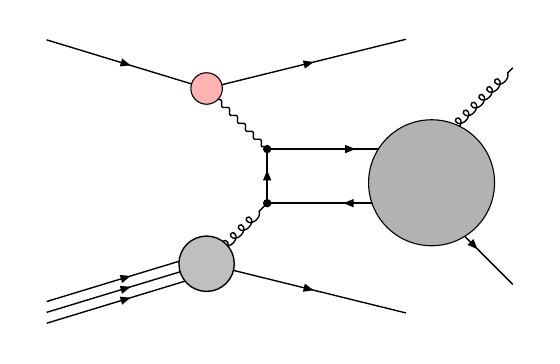
\begin{tikzpicture}
    \begin{feynhand}
  \node (root) at (0,0) {};

  \begin{scope}[on background layer]
    \node[dot] (dot1) [below = .05cm of root] {};

    \node[dot] (dot2) [below = 2.0cm of dot1] {};
    \node[dot] (dot3) [below = .05cm of dot2] {};
    \node[dot] (dot4) [below = .05cm of dot3] {};


    \node[] (ddot1) [above left = .5 and 2 of dot1] {};

    \node[] (ddot2) [below left = .5 and 2 of dot2] {};
    \node[] (ddot3) [below left = .5 and 2 of dot3] {};
    \node[] (ddot4) [below left = .5 and 2 of dot4] {};

    \node[] (ddot5) [above right = .5 and 2.5 of dot1] {};
    \node[] (ddot6) [below right = .5 and 2.5 of dot3] {};


    \node[dot] (middle1) [below right= 1cm of dot1] {};
    \node[dot] (middle2) [above right= 1cm of dot3] {};
    \node[dot] (pivot1) [right = 2cm of middle1] {};
    \node[dot] (pivot2) [right = 2cm of middle2] {};
    \node[dot] (pivot) [below=.34cm of pivot1] {};

    \node[] (ddot7) [above right = of pivot1] {};
    \node[] (ddot8) [below right = of pivot2] {};

    \propag[fer] (ddot1) to (dot1);
    \propag[fer] (ddot2) to (dot2);
    \propag[fer] (ddot3) to (dot3);
    \propag[fer] (ddot4) to (dot4);

    \propag[pho] (dot1) to (middle1);
    \propag[glu] (dot3) to (middle2);
    \propag[fer] (middle1) to (pivot1);
    \propag[antfer] (middle2) to (pivot2);
    \propag[antfer] (middle1) to (middle2);

    \propag[fer] (dot1) to (ddot5);
    \propag[fer] (dot3) to (ddot6);
    
    \propag[glu] (pivot1) to (ddot7);
    \propag[fer] (pivot2) to (ddot8);
  \end{scope}

  \vertex[grayblob] (blob1) at (dot3) {};

  \filldraw[fill=black!30!white] to (pivot) circle [radius=.8cm];
  \filldraw[fill=red!30!white] to (dot1) circle [radius=.2cm];
\end{feynhand}

  \end{tikzpicture}
\end{figure}

\begin{figure}[htb!]
  \centering
  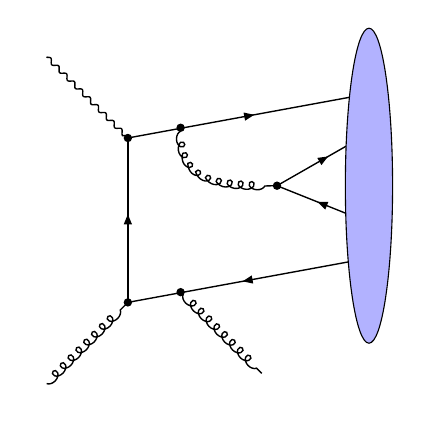
\begin{tikzpicture}
    \begin{feynhand}
  \node (root) at (0,0) {};
  \begin{scope}[on background layer]
    \vertex[dot] (vert1) at (root) {};
    \vertex[dot] (vert2) [below = 2 of vert1] {};

    \vertex[dot](vert3) [above right = .5 and 3 of vert1] {};
    \vertex[dot](vert4) [below = 2 of vert3] {};
    \vertex[dot](vert5) [below left = .37 and 2.33 of vert3]{};
    \vertex[dot](vert6) [below left = .37 and 2.33 of vert4]{};

    \node(dot1) [above left = of vert1] {};
    \node(dot2) [below left = of vert2] {};
    \node(pivot) [below = 1 of vert3] {};
    \node(dot3) [below right = of vert6] {};
    
    \vertex[dot] (split) [left = 1 of pivot] {};
    \vertex[dot] (splitup) [above = .5 of pivot] {};
    \vertex[dot] (splitdown) [below = .3 of pivot] {};

    \propag[pho] (dot1) to (vert1);
    \propag[glu] (dot2) to (vert2);
    \propag[antfer] (vert1) to (vert2);
    \propag[fer] (vert1) to (vert3);
    \propag[antfer] (vert2) to (vert4);
    \propag[glu] (vert5) to [out=270, in=180, looseness=1.2] (split);
    \propag[fer] (split) to (splitup);
    \propag[antfer] (split) to (splitdown);
    \propag[glu] (vert6) to (dot3);
  \end{scope}
  
  \filldraw[fill=blue!30!white] to (pivot) ellipse (.3cm and 2cm);
\end{feynhand}


  \end{tikzpicture}
\end{figure}

\begin{figure}[htb!]
  \centering
  \begin{tikzpicture}
    \begin{feynhand}
  \nood (root) at (0,0) {};
  
\end{feynhand}


  \end{tikzpicture}
\end{figure}

\vspace{10pt}

% --------------------------------------------- %
\bibliographystyle{acm}
\bibliography{referencias}
% --------------------------------------------- %
\end{document}


